This chapter will, step by step, introduce the sensors, describe how they function and define the methods used to extract the data from them. The accelerometer and gyroscope that we are using are both part of the built-in IMU of the Ardupilot, fitted on 6-axis MPU6000 14-bit chip. The accelerometer works by detecting a force that is actually the opposite of the acceleration vector. This force is not always caused by acceleration, but it can be. It just happens that acceleration causes an inertial force that is captured by the force detection mechanism of the accelerometer. The gyroscope measures the rotation around one of the axes.

\section{Accelerometer}
According to the MPU-6000 datasheet (ADD REFERENCE), the raw accelerometer data can be converted into multiples of \textit{g} by dividing with a factor of 16384. However, we have computed the rotations around the axes by using an alternative method. We have first chosen a reference position, which is the typical orientation of a device with the x and y axis in the 0 \textit{g} field plane and the x axis in the 1 \textit{g} field. This is shown in figure REF, where $\theta$ is the angle between the horizon and the x-axis of the accelerometer, $\psi$ as the angle between the horizon and the y-axis of the accelerometer, and
$\phi$ as the angle between the gravity vector and the z-axis. When in the initial position of \textit{0} g on the x- and y-axes and 1 \textit{g} on the z-axis, all calculated angles would be 0 degrees. ADD REF SAME AS PICTURE

\begin{figure}[H]
  \centering
    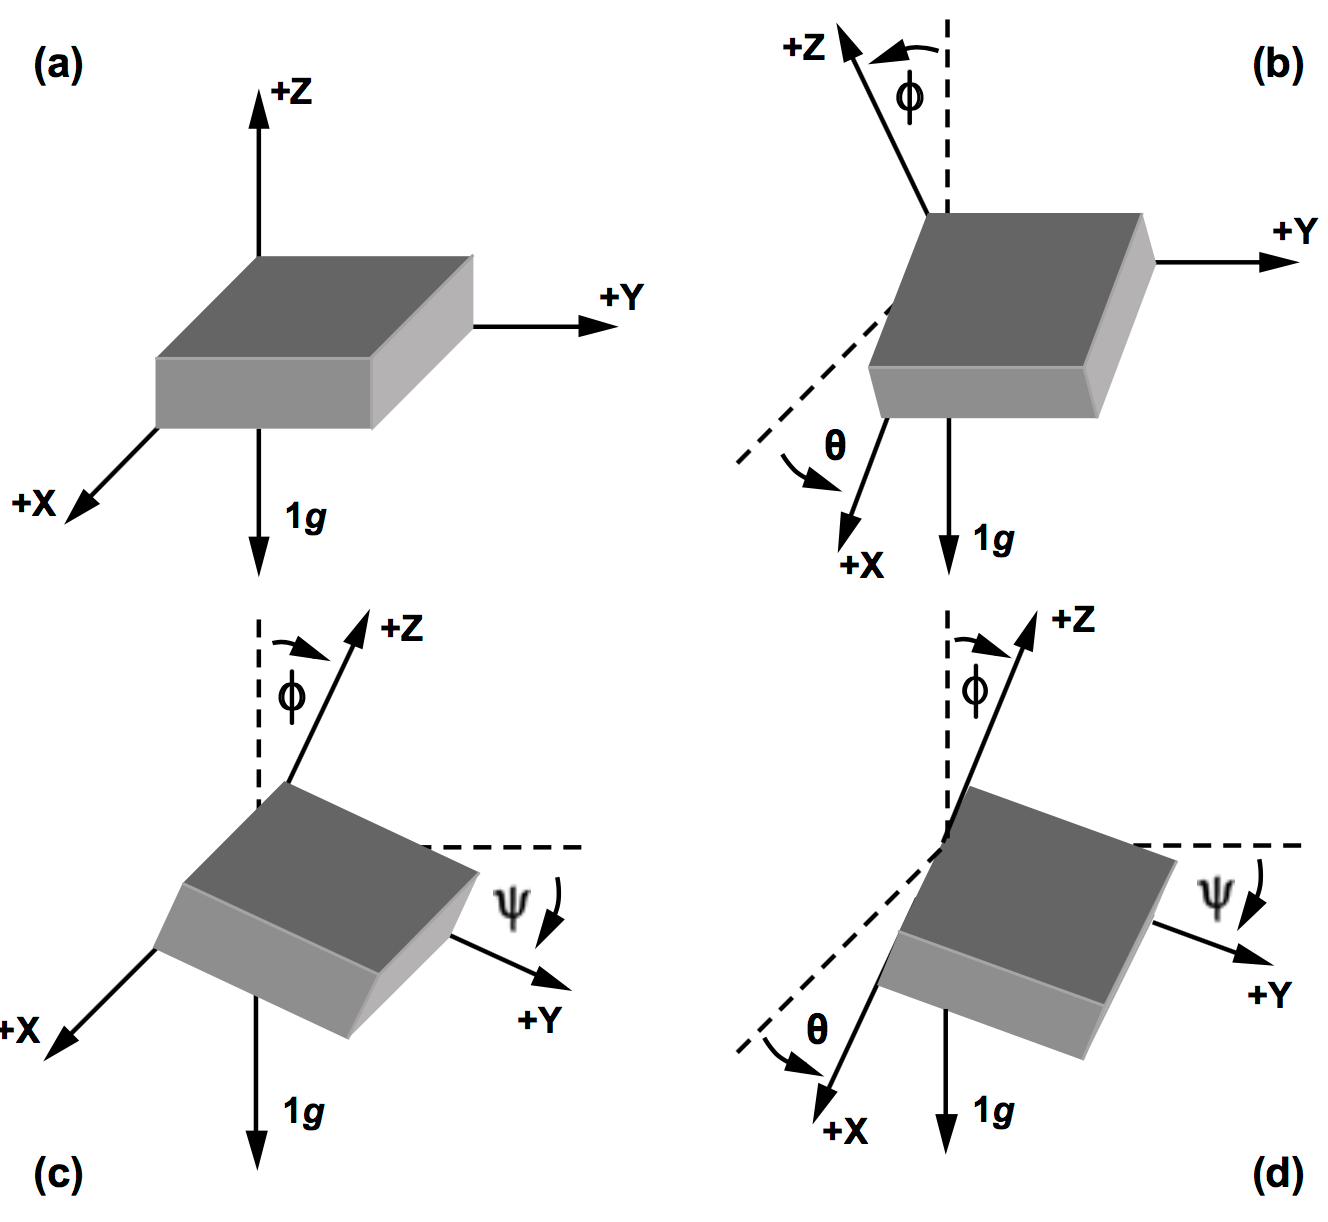
\includegraphics[width=0.8\textwidth]{images/accangle.png}
	\caption{Inclination angles //http://www.analog.com/media/en/technical-documentation/application-notes/AN-1057.pdf}
	\label{acc}
\end{figure} 
To measure the direction of the gravity vector and define the pitch and roll angles, an accelerometer is an easy to use solution.
The raw ADC values obtained from the accelerometer first have to be converted into some acceleration $m/s^2$. To make this happen, a resolution equation is defined that will describe the relationship between the raw values and the acceleration.
For this particular accelerometer, some general acceleration $a_\theta $ along some axis $\theta$ can be found using Equation \ref{sensors1}.

Therefore, by using basic trigonometry, the formulas for the converted accelarometer data are:

\begin{equation}	
 	\theta=tan^{-1}(\frac{A_{X}}{\sqrt{A_{Y}^{2}+A_{Z}^{2}}})
 \end{equation}
 
 \begin{equation}	
 	\psi=tan^{-1}(\frac{A_{Y}}{\sqrt{A_{X}^{2}+A_{Z}^{2}}})
 \end{equation}
 
 \begin{equation}	
 	\phi=tan^{-1}(\frac{\sqrt{A_{X}^{2}+A_{Y}^{2}}}{A_{Z}})
 \end{equation}
 
The inversion of the last equation is due to the initial position being a 1 \textit{g} field. If the horizon is desired as the reference for the z-axis, the operand can be inverted. A positive angle means that the corresponding positive axis of the accelerometer is pointed above the horizon, whereas a negative angle means that the axis is pointed below the horizon. Because the inverse tangent function and a ratio of accelerations is used, the benefits mentioned in the dual-axis example apply, namely that the effective incremental sensitivity is constant and that the angles can be accurately measured for all points around the unit sphere.

An important thing to keep in mind is that the accelerometer provides accurate orientation angles when gravity is the only force acting on the sensor. When manouvering the sensor, other forces are being applied to it, which causes a fluctuation in the measurements. As a result, the accelerometer provides accurate data over the long term, but is noisy in the short term. ADD REFERENCE http://www.geekmomprojects.com/gyroscopes-and-accelerometers-on-a-chip/

\section{Gyroscope}
Computing orientation from the gyroscope sensor is different, since the gyroscope measures angular velocity (the rate of change in orientation angle), not angular orientation itself. To compute the orientation, we must first initialize the sensor position, then measure the angular velocity $\omega$ around the X, Y and Z axes at measured intervals ($\Delta t$).   Then $\omega \times \Delta t$ is the change in angle. The new orientation angle will be the original angle plus this change. The problem with this approach is that we are integrating – adding up many small computed intervals – to find orientation.  Repeatedly adding up increments of  $\omega \times \Delta t$ will result in small systematic errors becoming magnified over time. This is the cause of gyroscopic drift, and over long timescales the gyroscope data will become increasingly inaccurate. In short, the gyroscope provides accurate data about changing orientation in the short term, but the necessary integration causes the results to drift over longer time scales.

The MPU-6000 datasheet (ADD REFERENCE) shows that dividing the raw gyroscope values by 131 gives angular velocity in degrees per second, which multiplied by the time between sensor readings, gives the change in angular position. If we save the previous angular position, we simply add the computed change each time to find the new value.


\section{Programming}
It is important to understand how the sensors can actually deliver us the data. Usually, they fall into two categories: analogue and digital. The one we are using is digital and it can be programmed using I2C, SPI or USART communication. We have decided on SPI and the setup code for it is shown below:

\lstinputlisting[language=C++, firstline=31, lastline=41, caption={Setup}, label={code:c1}]{Arduino/acc_gyro_only/acc_gyro_only.ino}

As we can see, the setup ends by calling the \textit{ConfigureMPU6000()} function:

\lstinputlisting[language=C++, firstline=195, lastline=224, caption={Function to configure chip}, label={code:c1}]{Arduino/acc_gyro_only/acc_gyro_only.ino}

Firstly, we need to get the raw values from both accelerometer and gyroscope and that is done by accessing their registers. We have made separate functions, which can be seen in Code REFERENCE, that read from the registers of the accelerometer and gyroscope and that return the raw values of each sensor. These functions are very similar, the only difference being the registers that are accessed to get the information needed. 

\lstinputlisting[language=C++, firstline=95, lastline=100, caption={Function that accesses registers and returns a raw value.}, label={code:c1}]{Arduino/acc_gyro_only/acc_gyro_only.ino}

\lstinputlisting[language=C++, firstline=95, lastline=140, caption={Functions that accesses the registers and returns raw values}, label={code:c1}]{Arduino/acc_gyro_only/acc_gyro_only.ino}

If we want to calculate the inclination of a device relative to the ground for example, we can calculate the angle between the force vector and one of the z-axis. We can do that by using the formulas in SECTION X and by degree conversion. The functions that take care of converting the raw values from both accelerometer and gyroscope are the following:

\lstinputlisting[language=C++, firstline=144, lastline=163, caption={Function to obtain angles based on the raw values of the accelerometer.}, label={code:c2}]{Arduino/acc_gyro_only/acc_gyro_only.ino}

\lstinputlisting[language=C++, firstline=167, lastline=193, caption={Function to obtain angles based on the raw values of the accelerometer.}, label={code:c3}]{Arduino/acc_gyro_only/acc_gyro_only.ino}

We have used the Serial Monitor within the Arduino IDE environment to read the outputs from both sensors and they seem to be accurate. The difference in the values of the accelerometer output is because accelerometers are more sensitive to noise and vibrations. The figure below shows the printed outputs at steady state, that is when the quadcopter is parallel to the ground.

The serial monitor was used to print out the the angles. At steady state, it yielded the results seen in Figure \ref{angles}.

\begin{figure}[H]
  \centering
    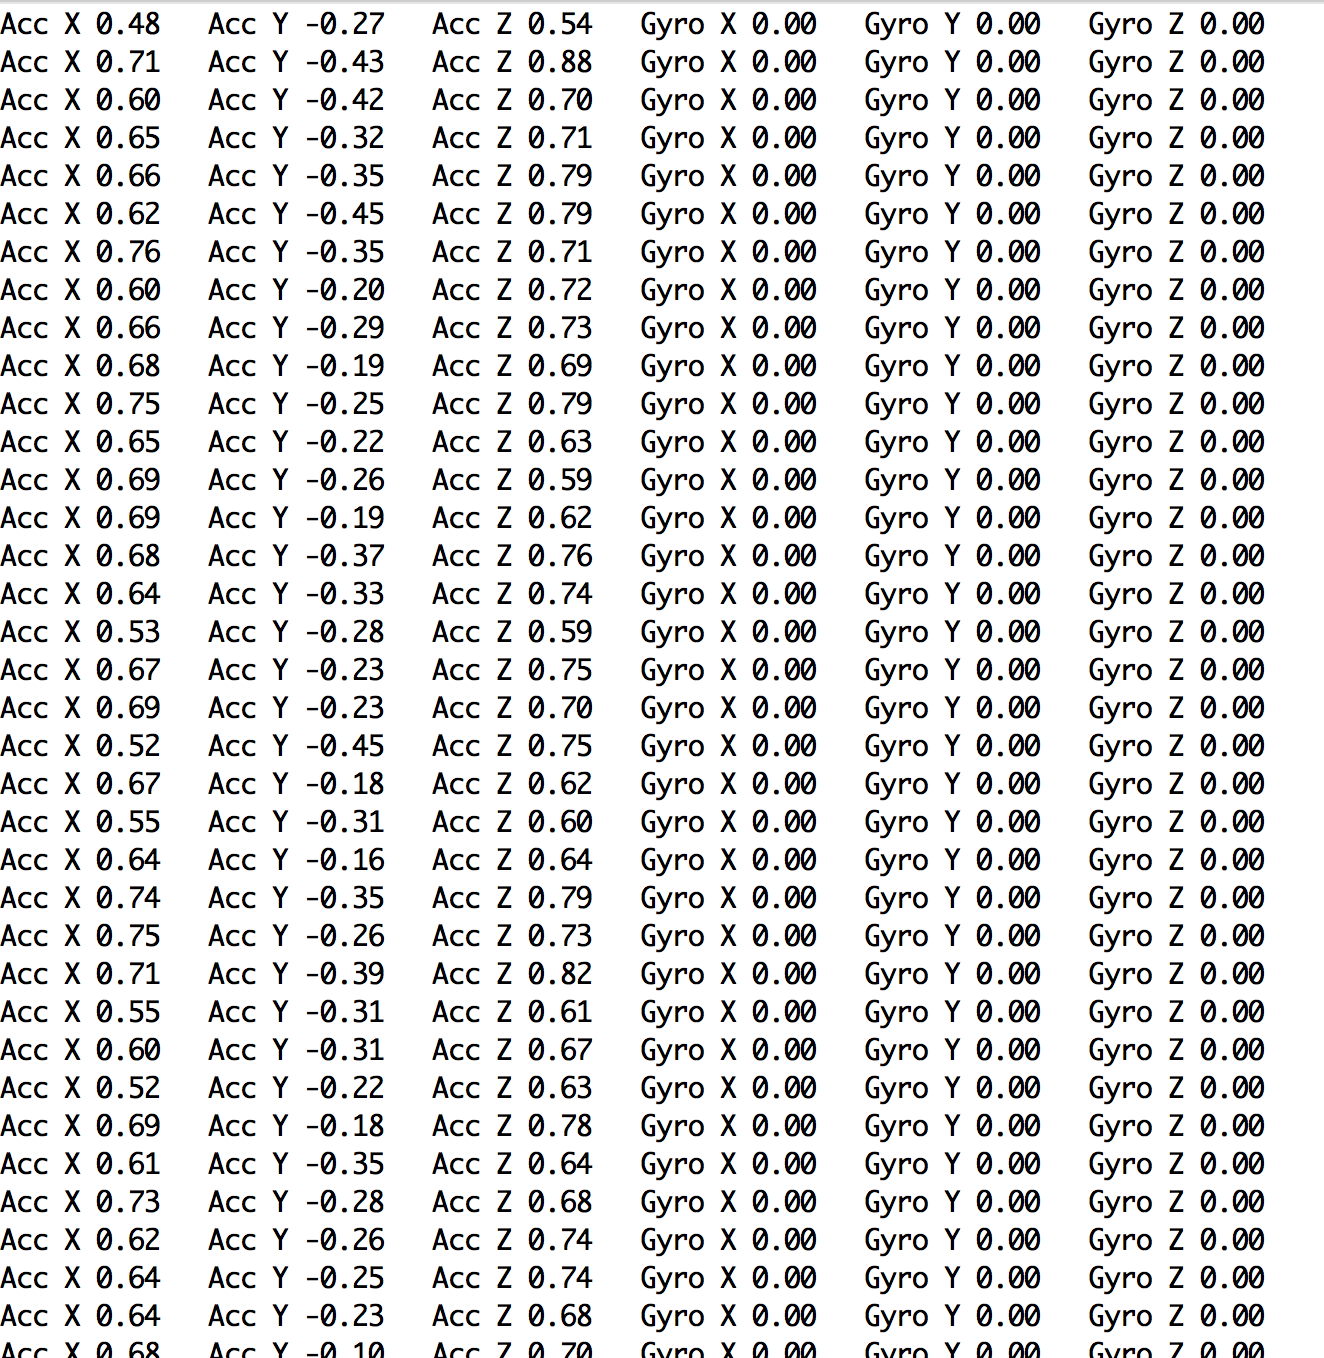
\includegraphics[width=1\textwidth]{images/accgy.png}
	\caption{Angles obtained from Accelerometer and Gyroscope.}
	\label{angles}
\end{figure}

//insert prinscreen for tilting 

\section{Filtering sensor data}
The configuration for the accelerometer and gyroscope enables a low-pass filter at 42Hz. However, looking at the data that the accelerometer reads, there is still some considerable amount of noise and occasional spikes in a steady state. In order to design a filter to counter these problems, flight of the prototype had to be simulated, to record the sensor values when the vehicle goes up in the air and tires to stabilize itself. Therefore, flight controller was unmounted from the frame, connected to a computer and then raised in the air, while tilting it to the sides. The test ran for 30 seconds and provided a $4591\times 6$ matrix, containing 4591 readings for all 3 axis of accelerometer and gyroscope. The plotted data over time for x-axis of the accelerometer and gyroscope can be seen in Figure \ref{dataPlot}.

\begin{figure}[H]
  \centering
    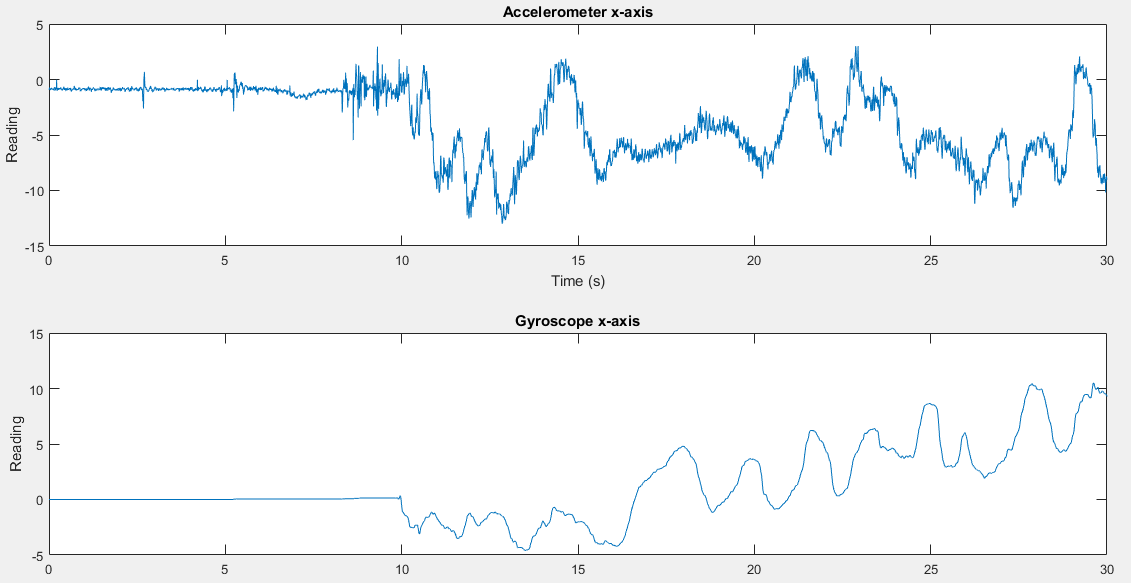
\includegraphics[width=1\textwidth]{images/MPUXPlot.png}
	\caption{Accelerometer and gyroscope x-axis test results.}
	\label{dataPlot}
\end{figure}

The sensor is running at approximately $\frac{4591}{30s} = 153Hz$ frequency, making any additional filter more difficult to perform. However, looking at the test data, it is evident that gyroscope provides clean results just with the help of on-board filter. The main focus then shifts towards the accelerometer - looking at the spectrogram of the accelerometer x-axis data (see Figure \ref{spectrogram}, a low-pass FIR filter is chosen.

\begin{figure}[H]
  \centering
    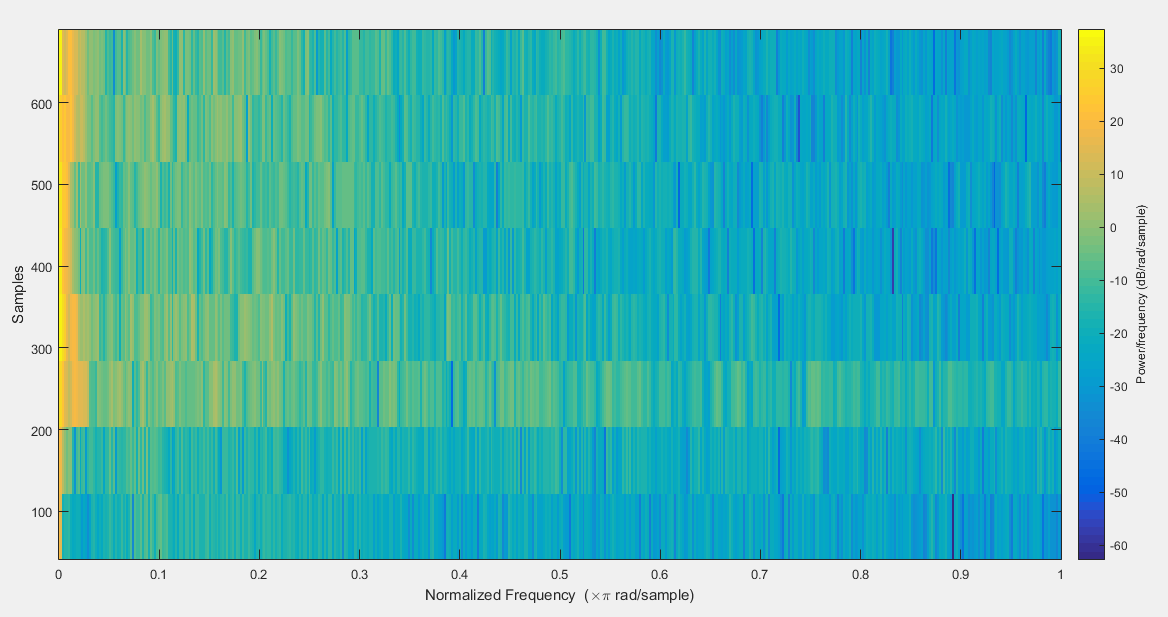
\includegraphics[width=1\textwidth]{images/spectrogram.png}
	\caption{Accelerometer x-axis spectrogram.}
	\label{spectrogram}
\end{figure}

In order to get rid of as much noise as possible, the cut-off frequency was chosen to be the maximum possible value - half of the sampling frequency. The order for the filter was chosen to be 10, mostly through trial and error - at this point, the filter has considerable effect, while not having a very high order, which carries its own cost. The filter was applied to the signal using simple code in Matlab, seen in Listing \ref{code:c4}.

\lstinputlisting[language=Matlab, firstline=1, lastline=6, caption={Filter generation code.}, label={code:c4}]{Arduino/AccelFilter.txt}

The filter was proven to be quite efficient, as seen in Figure \ref{accelFilter}. While not completely perfect, possible improvements will be covered in the discussion chapter.

\begin{figure}[H]
  \centering
    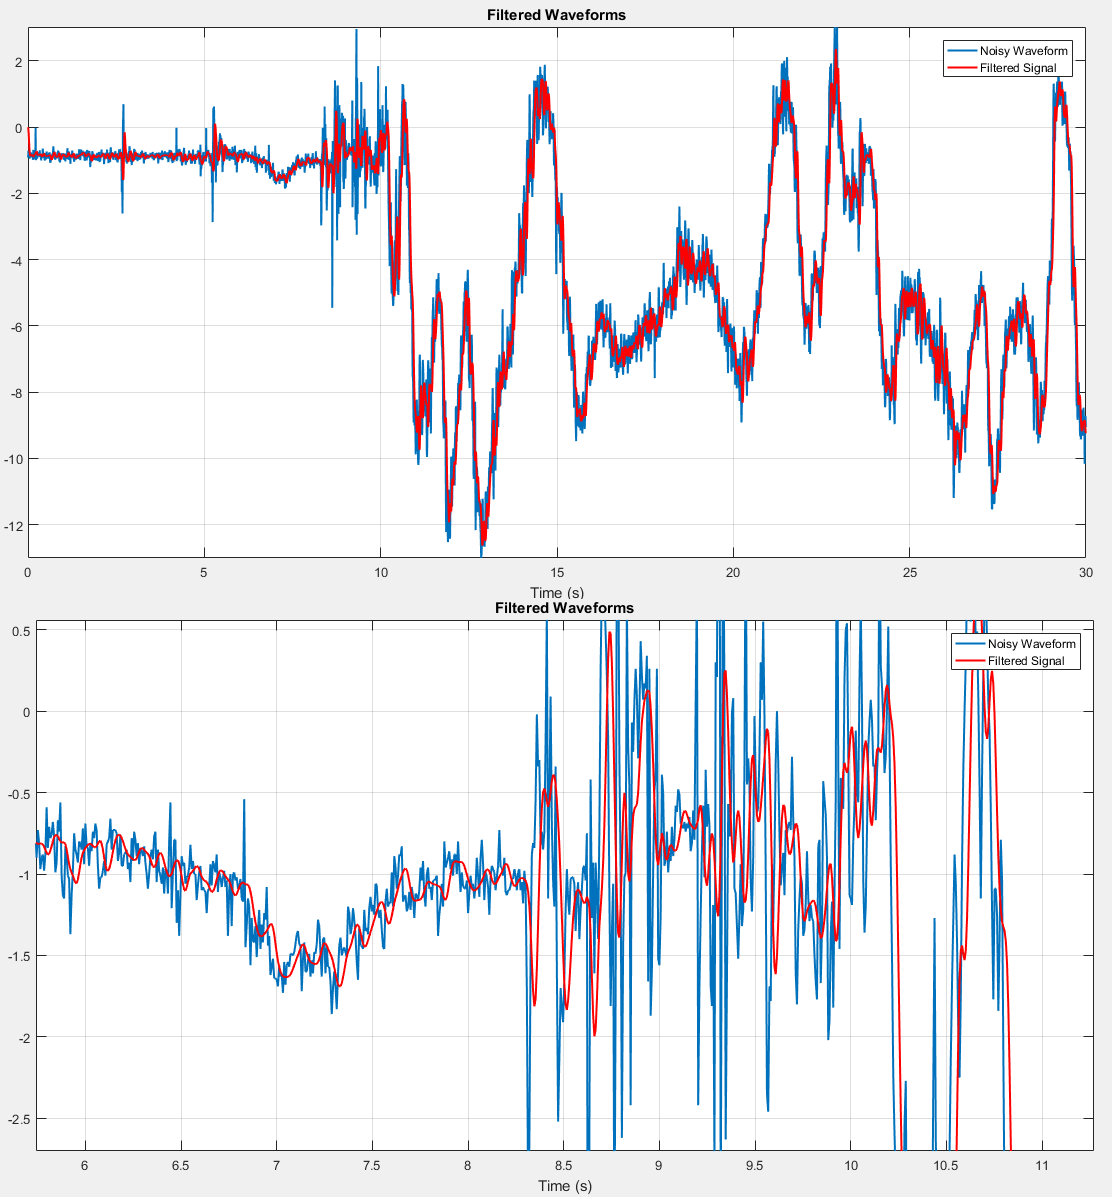
\includegraphics[width=1\textwidth]{images/accelFilter.png}
	\caption{Implemented filter and its close-up.}
	\label{accelFilter}
\end{figure}

%ULTRASONIC NO FILTER <- is it even necessary?